\section{Limitations of the Reactive Flux Approach}
\label{sec:limit}

Using the TST rate constants to describe the dynamics in terms of the master equation faces two main problems.
First, a strong dependence on the dividing surface cannot be corrected by a transmission coefficient if the boxes touch, since then $\kappa \equiv 1$.
Second, the evolutions (\ref{eq:A-to-B-a-of-t}) and (\ref{eq:A-to-B-and-back-a-of-t}) may depend on internal barriers which are disregarded in the TST approach.

\subsubsection*{Roughness of the Dividing Surface}

In TST, the rate constant, which should be an average over the whole box defining the reactants, strongly depends on the dividing surface, which represents only a small subset of the ensemble.
Miller argues\cite{Miller1976} that using the characteristic function $\chi$ for the reaction, the TST rate constant does not depend on the dividing surface.
However, he does not explicitly discuss the definition of species.
From the possibility of many dividing surfaces it follows that species are not defined as touching boxes in configuration or phase space, as there must be a sufficient gap allowing decorrelation.


\begin{figure}[htb]
\centering
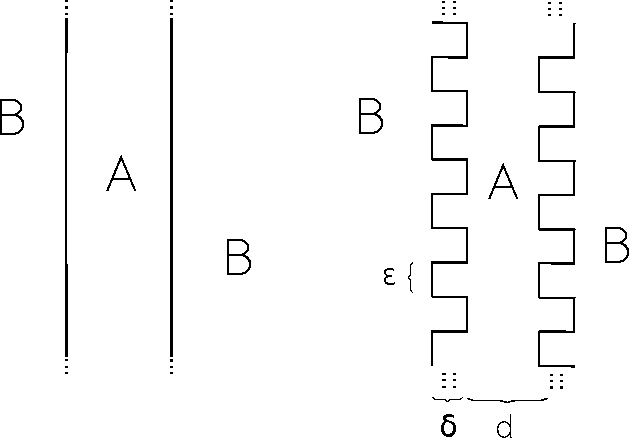
\includegraphics[width=8cm]{Images/diag3.pdf}
\caption[Effect of surface roughness on the rate constant.]{\textbf{Left:} box A with a smooth dividing surface between A and B. \textbf{Right:} box A with a rough dividing surface between A and B. $k^{TST}_{\rm A\rightarrow B}$ will be higher, even if $\delta \ll d$. }
\label{fig:rough}
\end{figure}

To illustrate the effect of a rough dividing surface on the dynamics, let us discuss two systems.
First, let us divide a plane into boxes A and B by two parallel lines of infinite potential (Figure \ref{fig:rough} left).
Without loss of generality, let the potential energy be everywhere constant in A, $\mathscr{V} \equiv 0$.
A point particle moving in A with velocity $u$ will bounce from either of the walls approximately once in time $t = d / u$, where $d$ is the width of box A.
Now let us increase the roughness (and therefore the length) of the dividing surface by lamellae of length $\delta \ll d$ and width $\varepsilon \ll \delta$.
We will observe a series of many (roughly $2 \delta / \varepsilon$) bounces separated in time by $t' = \varepsilon / u$ once in $t = d / u$.
The number of hits per time unit and therefore the apparent reactive flux will be much higher, but the real evolution of the system should not change since the change in the definition of species was negligible.

\subsubsection*{The Effect of Internal Barriers}

In region A we can define any number of internal dividing surfaces.
Trajectories starting from states far from the boundary of A must cross many of these inner surfaces, and these crossings and these crossings could correspond to a much slower process than the crossing of $\partial \rm AB$.
Region A can contain internal barriers (energetic or entropic, such as spacial bottlenecks or mazes, see figure \ref{fig:maze}).
Hence the mean passing time through the region can be higher than the time needed for crossing the final barrier.
The equilibrium rate constant does not need to include these effects.
However, in a description of real dynamics, this neglect is equivalent to the assumption that the flux through the dividing surface is the rate-determining event of the whole transition.

\begin{figure}[htb]
\centering
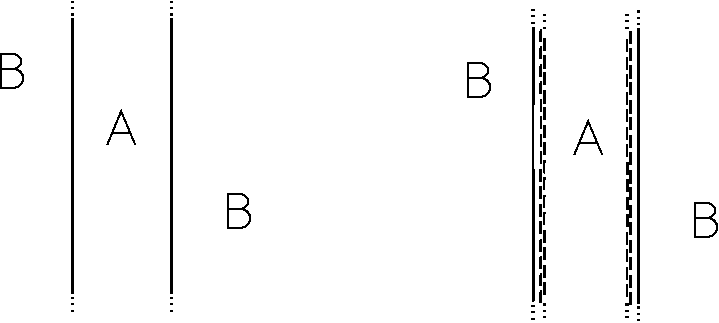
\includegraphics[width=9cm]{Images/diag1-2.pdf}
\caption[Comparison of systems with and without internal barriers.]{\textbf{Left:} box A without an internal barrier, where crossing the outer dividing surface may be the rate limiting step. \textbf{Right:}  box A with an internal barrier (maze) with a low probability of crossing.}
\label{fig:maze}
\end{figure}


